\section{Case Study of Law Graph}
\label{sec:a}
In this section, we apply the proposed law graph construction process in Section~\ref{con} to parse the Crime of Loan Fraud, Article 193 of the Criminal Law of China (shown in Table \ref{tab:three}), into a law graph.

\begin{figure}[H]
    \centering
    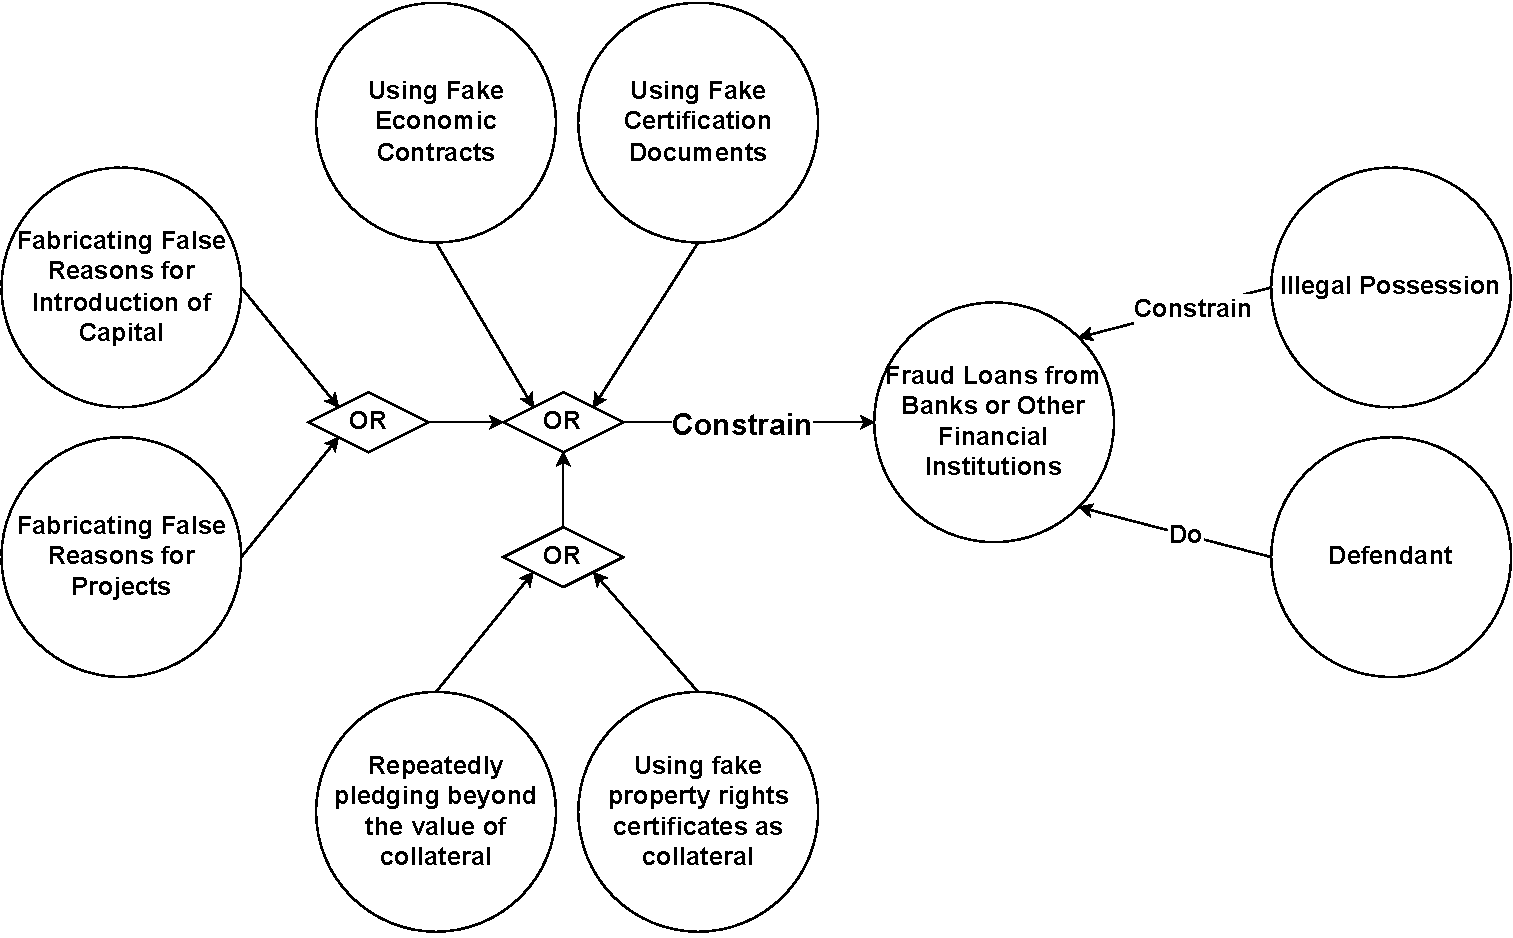
\includegraphics[width=1\linewidth]{figs/HP-Result.pdf}
    \caption{Result of Hypothesis Parser on the Crime of Loan Fraud}
    \label{fig:HP-Result}
\end{figure}

\textbf{Hypothesis Parser (HP).} In terms of \textit{hypothesis}, the target is to find the illegal conduct (\( I \)) and any related conditions (\( M \)) of the conduct in the statutory provision. For the example in Table \ref{tab:three}, we obtain the following vertices and edges:
% with Algorithm \ref{alg:HP}:
\begin{itemize}
    \item Conduct Node $A$: \textit{Fraud Loans from Banks or Other Financial Institutions}
    \item Defendant Node $D$: \textit{Defendant}
    \item Motivation Node $M_v$: \textit{Illegal Possession}
    \item Other Conditions $M_o$: \textit{Using Fake Certification Documents}; \textit{Using Fake Economic Contracts}; \textit{Fabricating False Reasons for Introduction of Capital}; \textit{Fabricating False Reasons for Projects}; \textit{Repeatedly pledging beyond the value of collateral}; and \textit{Using fake property rights certificates as collateral}.
\end{itemize}

\begin{figure}[H]
    \centering
    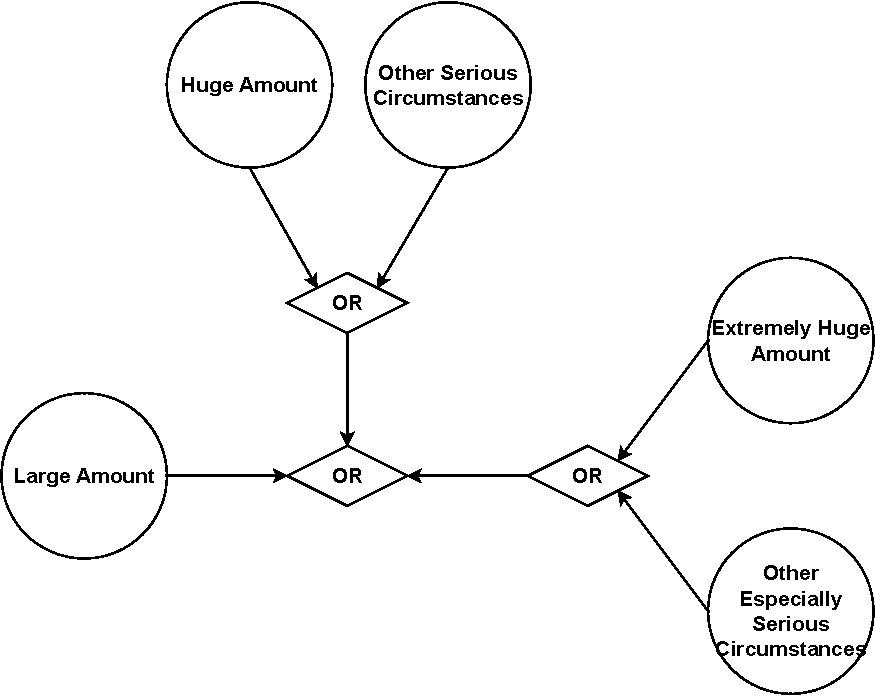
\includegraphics[width=1\linewidth]{figs/DP-Result.pdf}
    \caption{Result of Disposition Parser on the Crime of Loan Fraud}
    \label{fig:DP-Result}
\end{figure}

\textbf{Disposition Parser (DP).} 
% As is outlined in Algorithm \ref{alg:DP}, disposition 
The parser aims to extract all severity information from the statutory law. For the example in Table \ref{tab:three}, we obtain the following vertices and edges:

\begin{itemize}
    \item $D_1$: \textit{Large Amount}
    \item $D_2$: \textit{Huge Amount} OR \textit{Other Serious Circumstances}
    \item $D_3$: \textit{Extremely Huge Amount} OR \textit{Other Especially Serious Circumstances}
\end{itemize}


\begin{figure}[H]
    \centering
    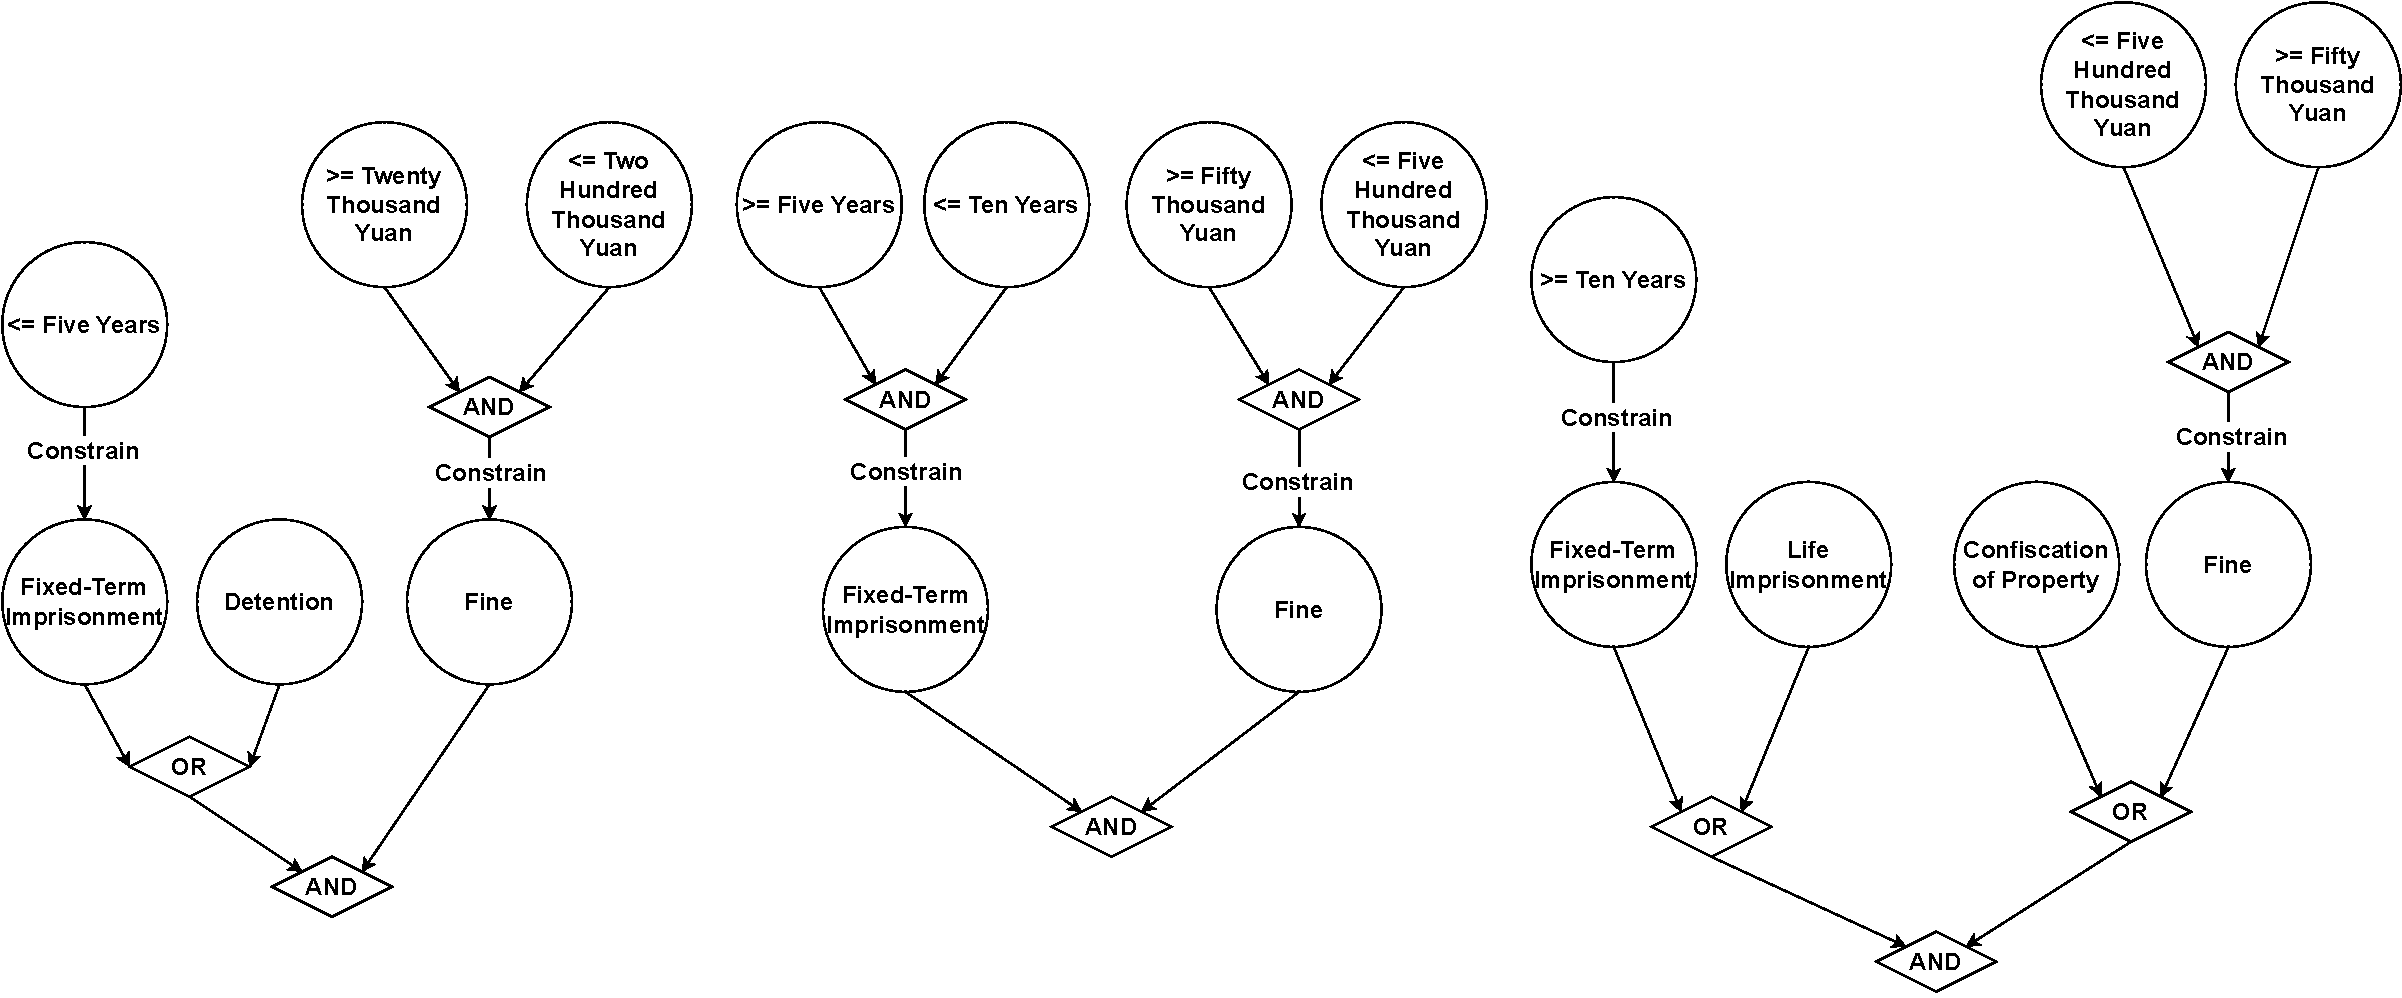
\includegraphics[width=1\linewidth]{figs/SP-Result.pdf}
    \caption{Result of Sanction Parser on the Crime of Loan Fraud}
    \label{fig:SP-Result}
\end{figure}

\begin{figure*}
    \centering
    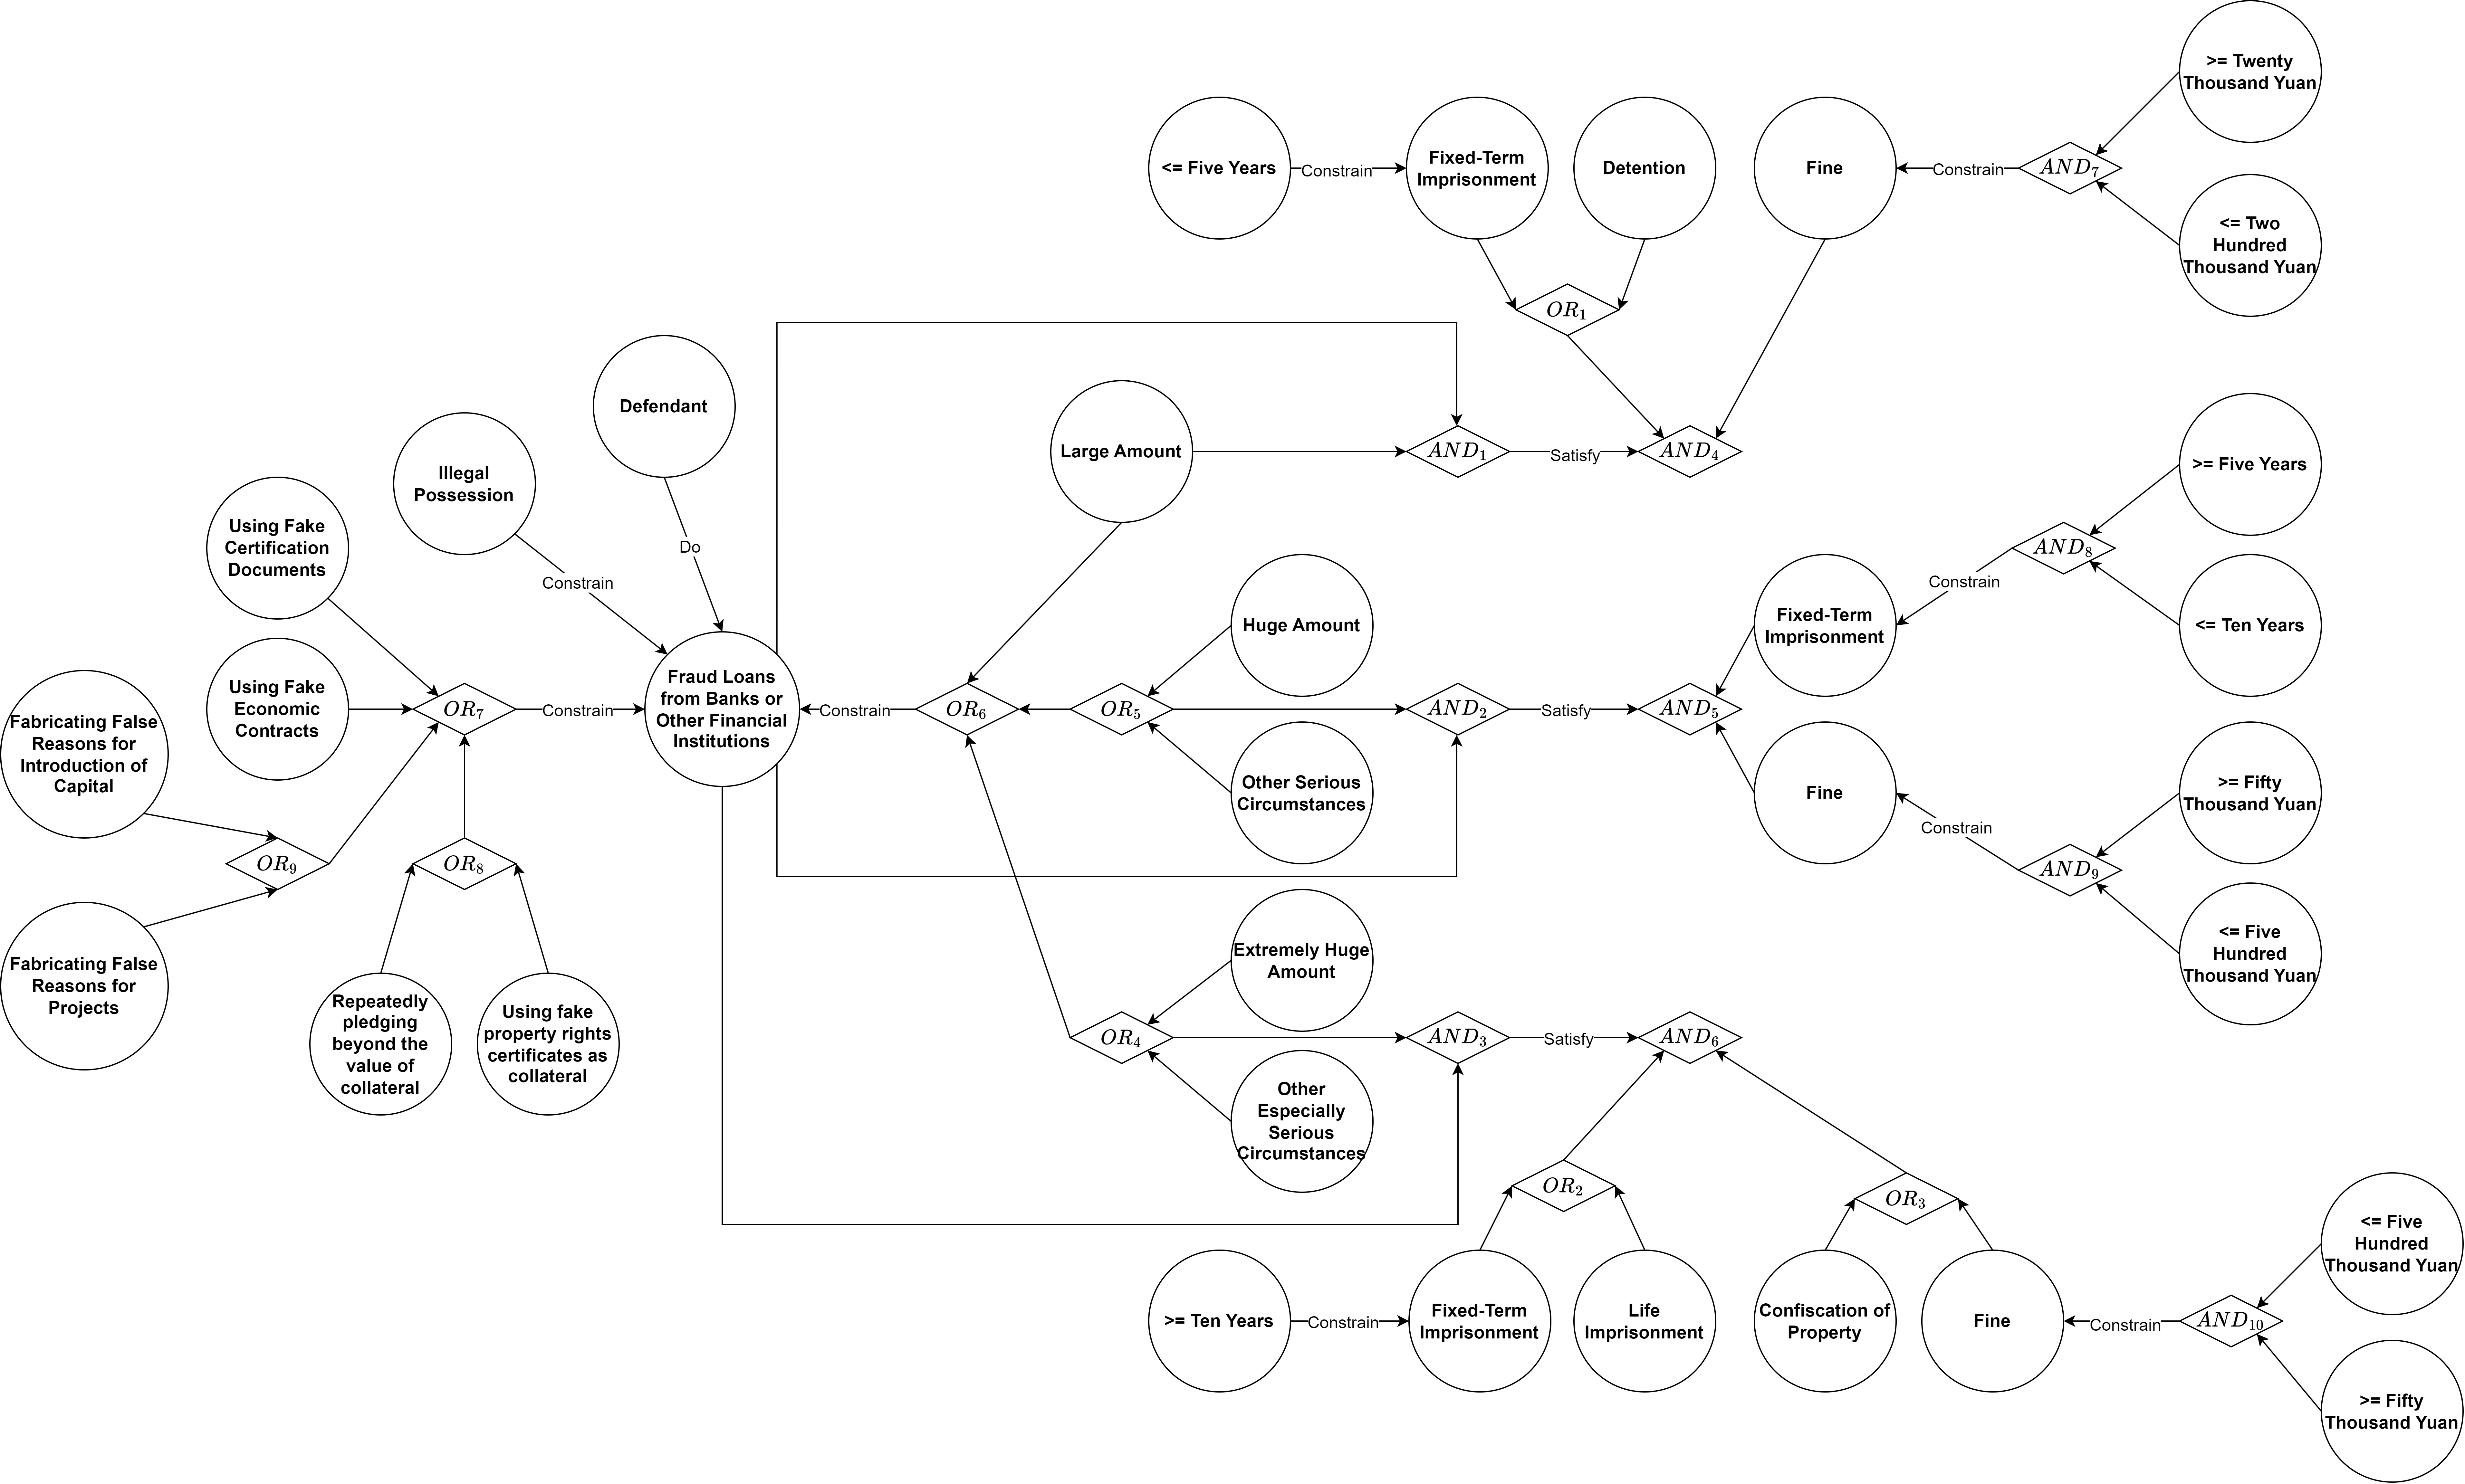
\includegraphics[width=0.98\linewidth]{figs/Loan Fraud Law Graph.png}
    \caption{Law-Graph on Crime of Loan Fraud}
    \label{Law-Graph-Case-study}
    \vspace{-1em}
\end{figure*}

\textbf{Sanction Parser (SP).}  
% Algorithm \ref{alg:SP} shows the process that .
SP parses all sanctions into \lawgraph{}. In this example, we obtain the following vertices and edges:
\begin{itemize}
    \item $P_1$: \textit{Fixed-term Imprisonment};
    \item $P_2$: \textit{Detention};
    \item $P_3$: \textit{Fine};
    \item $P_4$: \textit{Fixed-term Imprisonment};
    \item $P_5$: \textit{Fine};
    \item $P_6$: \textit{Fixed-term Imprisonment};
    \item $P_7$: \textit{Life Imprisonment};
    \item $P_8$: \textit{Fine};
    \item $P_9$: \textit{Confiscation of Property};
    \item $U_1$ and $L_1$: \textit{$\leq$ Five Years},  Not applicable;
    \item $U_2$ and $L_2$: Not applicable, Not applicable;
    \item $U_3$ and $L_3$: \textit{$\leq$ Two Hundred Thousand Yuan}, \textit{$\geq$ Twenty Thousand Yuan};
    \item $U_4$ and $L_4$: \textit{$\leq$ Ten Years}, \textit{$\geq$ Five Years};
    \item $U_5$ and $L_5$: \textit{$\leq$ Five Hundred Thousand Yuan};, \textit{$\geq$ Fifty Thousand Yuan};
    \item $U_6$ and $L_6$: Not applicable, \textit{$\geq$ Ten Years};
    \item $U_7$ and $L_7$: Not applicable, Not applicable;
    \item $U_8$ and $L_8$: \textit{$\leq$ Five Hundred Thousand Yuan}, \textit{$\geq$ Fifty Thousand Yuan};
    \item $U_7$ and $L_7$: Not applicable, Not applicable.
\end{itemize}




After obtaining these nodes, we utilize the edge definition (Table~\ref{tab:edge})
% and Algorithm \ref{alg:HP} to \ref{alg:Integration} 
to connect these nodes. Then, we can get the complete law graph of the Crime of Loan Fraud, Article 193 of the Criminal Law of China, shown in Figure~\ref{Law-Graph-Case-study}. After construction, we can identify the source nodes and output nodes in the \lawgraph{}, including
\begin{itemize}
    \item Source nodes: \textit{Large Amount}, \textit{Huge Amount}, \textit{Other Serious Circumstances}, \textit{Extremely Huge Amount}, \textit{Other Especially Serious Circumstances}, \textit{Defendant}, \textit{Illegal Possession}, \textit{Using Fake Certification Documents}, \textit{Using Fake Economic Contracts}, \textit{Fabricating False Reasons for Introduction of Capital}, \textit{Fabricating False Reasons for Projects}, \textit{Repeatedly pledging beyond the value of collateral}, and \textit{Using fake property rights certificates as collateral};
    \item Output nodes: \textit{AND$_1$}, \textit{AND$_2$}, and \textit{AND$_3$}.
\end{itemize}




